\documentclass[11pt,a4paper,twoside]{article}
\usepackage{a4}
\usepackage[left=2cm,right=2cm,top=2.5cm,bottom=2.5cm,includeheadfoot]{geometry}
\usepackage[english]{babel}
%------------------------------- blindtex
\usepackage[pangram]{blindtext}
%------------------------------- color
\usepackage{color}
%------------------------------- math
\usepackage{amsfonts}
\usepackage{amstext}
\usepackage{amsmath}
%------------------------------- Graphics
\usepackage{graphics}
\usepackage{graphicx}
\usepackage{picinpar}
\usepackage{floatflt}
%------------------------------- 
\usepackage{csquotes}
\usepackage{url}
%------------------------------- Index   
\usepackage{makeidx}

\addto{\captionsenglish}{%
  \renewcommand{\indexname}{Index}
}

\makeindex
%------------------------------- Bib latex for references  
\usepackage[backend=biber,
            style=numeric,
            natbib=true,
            sortlocale=de_DE,
            doi=true,
            eprint=false
            ]{biblatex}
\addbibresource{literature.bib}	% bib file
\defbibheading{lit}{\section{Bibliography}}
%------------------------------- info
\usepackage[]{hyperref}	
\hypersetup{pdfauthor={K.D.T.S.},%
            pdftitle={Testing the latexCompiler},%
            pdfproducer={LaTeX},%
            pdfcreator={laTexCompiler.sh}
}
%------------------------------- SVG file embeding 
\newcommand{\executeiffilenewer}[3]{%
\ifnum\pdfstrcmp{\pdffilemoddate{#1}}%
{\pdffilemoddate{#2}}>0%
{\immediate\write18{#3}}\fi%
}
\newcommand{\includesvg}[1]{%
\executeiffilenewer{#1.svg}{#1.pdf}%
{inkscape -z -D --file=#1.svg %
--export-pdf=#1.pdf --export-latex}%
\input{#1.pdf_tex}%
}

%------------------------------- start
\begin{document}


\section{LaTexCompiler v0.0.4}

	\textit{laTexCompiler.sh} is a short shell script written by KDTS (Kossi D. T. Saka).
	It is designed to compile a latex-document and generate a pdf-document using \"pdflatex\".\newline

	\begin{itemize}
		\item It can run/load a \textit{gnuplot}\index{Gnuplot} file to plot images that are inserted in the latex document. This requires \textit{gnuplot} to be installed.
		\item It can run \textit{biber}\index{Biber} to insert references from a \textit{biblatex}\index{Biblatex} document in the latex document, section 2. This requires \textit{biber} to be installed.
		\item It can generate the \textit{index}\index{Index} page for the pdf document, page~5.
		\item It can compile a latex-document that includes SVG images \cite{svgInLatex}, (figure \ref{fig:svgimg}) . It may be necessary to installe \textit{inkscape}\index{Inkscape}.
		\item It clears\index{Clear} by default unnecessary documents like *(.aux, .out, .toc, .bcf ....).
	\end{itemize}


	\subsection{Keep it simple}
		the first objective of the program is to make it as easy as possible to generate pdf document from latex file without writing much command. 
		To achieve this simplicity proceed as follow 
		\begin{enumerate}
			\item open the script to edit the CONFIGURATION PART (lines 14 - 39)
			\item follow the instractions to enter the name (and location path)  of your documents
			\item save the changes
		\end{enumerate}
		That's it. NOW YOU CAN JUST CALL \textcolor{blue}{\textit{./laTexCompiler.sh}}\\
		 It's that simple!

	\subsection{Some commands}

	\begin{description}
		\item[Generate pdf-document simple:]$\,$\\ 
			 \textcolor{blue}{\textit{./laTexCompiler.sh} -t texDocument.tex}\\
			 in the case that the latex document is not located in the same directory as the script:\\
			 \qquad\textcolor{blue}{\textit{./laTexCompiler.sh} -t /path/to/texDocument.tex} (if you are in the directory where the script is located)
			 \qquad or \\
			 \qquad\textcolor{blue}{\textit{./path/to/laTexCompiler.sh} -t texDocument.tex} (if you are in the directory where the latex document is located)

		\item[Load gnuplot file WITHOUT generating pdf-document]$\,$\\ 
			\textcolor{blue}{\textit{./laTexCompiler.sh} -p plot.tpl}

		\item[Load gnuplot file AND generate pdf-document including images]$\,$\\ 
			\textcolor{blue}{\textit{./laTexCompiler.sh} -t texDocument.tex -p plot.tpl}

		\item[Generate pdf-document AND insert references]$\,$\\ 
			\textcolor{blue}{\textit{./laTexCompiler.sh} -t texDocument.tex -b biblatexDocument.bib}

		\item[Generate pdf-document BUT do not clear file like *(.aux, .out, .toc, .bcf ....)]$\,$\\
			\textcolor{blue}{\textit{./laTexCompiler.sh}  -t texDocument.tex -{}-clear no}

		\item[Extended command]$\,$\\ 
			\textcolor{blue}{\textit{./laTexCompiler.sh} -t texDocument.tex -b biblatexDocument.bib -p plot.tpl -{}-svg -{}-index}\\
			It loads gnuplot file; generates pdf-document including images as well as SVG images; inserts references AND creates the index.

	\end{description}

	
	\subsection{Options}
	 
	\hspace*{-1.3cm}\begin{tabular}{lll}
		\textbf{Command} & \textbf{Alternative Command} & \textbf{Description}\\
		\hline\hline	
		 \textcolor{blue}{-h}          	 & \textcolor{blue}{-{}-help}               		& Display the help\\ 
		 \hline
		 \textcolor{blue}{-t} $<$file$>$\footnotemark[1]   & \textcolor{blue}{-{}-texfile} $<$file$>$\footnotemark[1]    	& Compile latex document\\ 
		 \hline
		 \textcolor{blue}{-p} $<$file$>$\footnotemark[1]   & \textcolor{blue}{-{}-plotfile} $<$file$>$\footnotemark[1]     	& Compile gnuplot-file to plot images for the latex document\\ 
		 \hline
		 \textcolor{blue}{-b} $<$file$>$\footnotemark[1]   & \textcolor{blue}{-{}-bibfile} $<$file$>$\footnotemark[1]      	& Bind biblatex-file to integrate references\\ 
		 \hline
		 \textcolor{blue}{-s}          	 & \textcolor{blue}{-{}-svg}                		& Compile tex-file regarding SVG images\\ 
		 \hline
		 \textcolor{blue}{-i}          	 & \textcolor{blue}{-{}-index}               		& Make index page\\ 
		 \hline
		 \textcolor{blue}{-c} [yes$|$no] 	 & \textcolor{blue}{-{}-clear} [yes$|$no]      	& Remove unnecessary like *(.aux, .out, .toc, .bcf ....) :: by default yes\\ 
		 \hline
	\end{tabular}

	\footnotetext[1]{$<$file$>$ or $<$/path/to/file$>$ depending on where the file is situated relative to the script.}

	\subsection{Inserted image using laTexCompiler.sh}
		\begin{figure}[!h]
		   \centering
		 	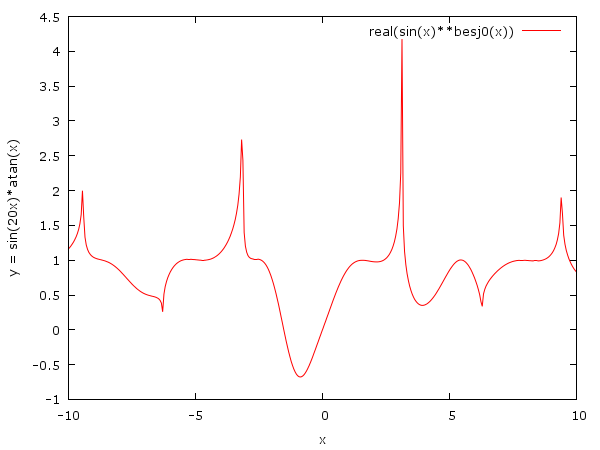
\includegraphics[width=12cm]{nameOfTheImage.png}
		 	\caption{This is the caption 1.}
		\end{figure}

	\subsection{Inserted SVG image using laTexCompiler.sh}
		\begin{figure}[!h]
		     \centering
		     \def\svgwidth{12cm}
		     \includesvg{svgImage}
		     \caption{This is the caption 2.}
		     \label{fig:svgimg}
		\end{figure}

	\subsection{Using references}
	The five boxing wizards jump quickly \cite{schwarz2011numerische}. Sympathizing would fix Quaker objectives. Many-wived Jack laughs at probes of sex quiz. Turgid saxophones blew 
	over Mick’s jazzy quaff. Playing jazz vibe chords quickly excites my wife. A large fawn jumped quickly over white zinc boxes \cite{rieg2014finite}. Exquisite farm wench gives body 
	jolt to prize stinker. Jack amazed a few girls by dropping the antique onyx vase! The quick brown fox jumps over the lazy dog. Jackdaws love my big Sphinx of 
	Quartz \cite{kaballo2011grundkurs}.
	%\Blindtext[1][3]


\clearpage
\printbibliography[heading=lit]\label{sec:literature}

\clearpage
\printindex\label{sec:indexed}

\end{document}
